%%%%%%%%%%%%%%%%%%%%%%%%%%%%%%%%%%%%%%%%%%%%%%%%%%%%%%%%%%%%%%%%%%%%%%%
%                                                                     %
%	Anomalous Diffusion in 1D Disordered Systems				      %
%                                                                     %
%%%%%%%%%%%%%%%%%%%%%%%%%%%%%%%%%%%%%%%%%%%%%%%%%%%%%%%%%%%%%%%%%%%%%%%

%%%%%%%%%%%%%%%%%%%%%%%%%%%%%%%%%%%%%%%%%%%%%%%%%%%%%%%%%%%%%%%%%%%%%%%
%% Preamble                                                           %
%%%%%%%%%%%%%%%%%%%%%%%%%%%%%%%%%%%%%%%%%%%%%%%%%%%%%%%%%%%%%%%%%%%%%%%

%% The preamble tells the program that you are using how to set up the 
%% document and calls any necessary packages. The packages that you
%% load are determined based on what you want to do. That means, you
%% typically will not load (or even know about) a package until you
%% need it. The following preamble should allow you to do many of the
%% things you may want to do.

%\documentclass[preprint,12pt]{elsarticle}

%% Use the option review to obtain double line spacing
%% \documentclass[authoryear,preprint,review,12pt]{elsarticle}

%% Use the options 1p,twocolumn; 3p; 3p,twocolumn; 5p; or 5p,twocolumn
%% for a journal layout:
\documentclass[final,1p,times]{elsarticle}
%% \documentclass[final,1p,times,twocolumn]{elsarticle}
%% \documentclass[final,3p,times]{elsarticle}
%% \documentclass[final,3p,times,twocolumn]{elsarticle}
%% \documentclass[final,5p,times]{elsarticle}
%% \documentclass[final,5p,times,twocolumn]{elsarticle}

%% The following lines allow for certain features in the document to
%% work. Do not worry about the ones called. If you do not use them
%% it won't hurt anything. If there are additional features that you
%% need, then you can load more packages just as below.

\usepackage{amsmath,amssymb,amsthm,amsfonts,blkarray,pgfplots,tkz-fct}
\usepackage{graphicx,color,epsfig,multimedia,epstopdf,caption,chngcntr}
\usepackage{verbatim,url}
\pgfplotsset{compat=1.11}
\usetikzlibrary{intersections,backgrounds,trees}
\biboptions{sort&compress}
\usepackage[T1]{fontenc}
\usepackage{float}

%% The following lines of code are self-made definitions to make 
%% calling certain commands easier (since I use them frequently). It
%% is not necessary to use any of these definitions.

\def\NN{\mathbb N} %Symbol for natural numbers
\def\ZZ{\mathbb Z} %Symbol for integers
\def\RR{\mathbb R} %Symbol for real numbers
\def\CC{\mathbb C} %Symbol for complex numbers

\everymath{\displaystyle}
\def\l{\left}
\def\r{\right}
\newcommand{\bb}[1]{\begin{equation}\label{#1}}
\newcommand{\ee}{\end{equation}}
\newcommand{\bbb}{\begin{eqnarray}}
\newcommand{\eee}{\end{eqnarray}}
\newcommand{\bbbb}{\begin{eqnarray*}}
\newcommand{\eeee}{\end{eqnarray*}}
\newcommand{\nnn}{\nonumber}
\newcommand{\no}{\noindent}
\def\R#1{$(\ref{#1})$}

\newtheorem{theorem}{Theorem}
\newtheorem{lemma}{Lemma}
\newtheorem{cor}{Corollary}
\theoremstyle{remark}
\newtheorem{remark}{Remark}
\theoremstyle{definition}
\newtheorem{definition}{Definition}

\makeatletter
\def\thmhead@plain#1#2#3{%
  \thmname{#1}\thmnumber{\@ifnotempty{#1}{ }\@upn{#2}}%
  \thmnote{ {\the\thm@notefont#3}}}
\let\thmhead\thmhead@plain
\makeatother

%% Colored comments

\newcommand{\josh}[1]{\textcolor{red}{\textbf{#1}}}
\newcommand{\conni}[1]{\textcolor{blue}{\textbf{#1}}}
\newcommand{\eva}[1]{\textcolor{green}{\textbf{#1}}}

%% The lineno packages adds line numbers. Start line numbering with
%% \begin{linenumbers}, end it with \end{linenumbers}. Or switch it on
%% for the whole article with \linenumbers.
%% \usepackage{lineno}

\journal{}

%%%%%%%%%%%%%%%%%%%%%%%%%%%%%%%%%%%%%%%%%%%%%%%%%%%%%%%%%%%%%%%%%%%%%%%
%% Beginning of Document                                              %
%%%%%%%%%%%%%%%%%%%%%%%%%%%%%%%%%%%%%%%%%%%%%%%%%%%%%%%%%%%%%%%%%%%%%%%

\begin{document}

\begin{frontmatter}

%% Title, authors and addresses

%% use the tnoteref command within \title for footnotes;
%% use the tnotetext command for theassociated footnote;
%% use the fnref command within \author or \address for footnotes;
%% use the fntext command for theassociated footnote;
%% use the corref command within \author for corresponding author footnotes;
%% use the cortext command for theassociated footnote;
%% use the ead command for the email address,
%% and the form \ead[url] for the home page:
%% \title{Title\tnoteref{label1}}
%% \tnotetext[label1]{}
%% \author{Name\corref{cor1}\fnref{label2}}
%% \ead{email address}
%% \ead[url]{home page}
%% \fntext[label2]{}
%% \cortext[cor1]{}
%% \address{Address\fnref{label3}}
%% \fntext[label3]{}

\title{Anomalous Diffusion in One-Dimensional Disordered Systems: A Discrete Fractional Laplacian Method}

%% use optional labels to link authors explicitly to addresses:
%% \author[label1,label2]{}
%% \address[label1]{}
%% \address[label2]{}

\author[ttu,ttu1]{J. L. Padgett}
\ead{joshua.padgett@ttu.edu}
\fntext[ttu]{Corresponding Author}
\address[ttu1]{Department of Mathematics and Statistics, Texas Tech University, Broadway and Boston, Lubbock, TX, 79409, USA}

\author[bu]{E. G. Kostadinova}
%\ead{eva_kostadinova@baylor.edu}

\author[bu,d]{C. D. Liaw}

\author[bu]{K. Busse}

\author[bu]{L. S. Matthews}

\author[bu]{T. W. Hyde}

\address[bu]{Center for Astrophysics, Space Physics, and Engineering Research and Department of Physics, One Bear Place, 97310, Baylor University, Waco, TX, 76706, USA}

\address[d]{Department of Mathematical Sciences, University of Delaware, 311 Ewing Hall, Newark, DE, 19716, USA}

\begin{abstract}
This work extends the study of Anderson-type Hamiltonians to include transport characterized by anomalous diffusion. 
%The current study introduces a novel model which employs the discrete fractional Laplacian, $(-\Delta)^s,\ s\in(0,2),$ and applies results from spectral and measure theory to study the occurrence of localization within a one-dimensional system.
Herein we investigate the occurrence of localization within a one-dimensional disordered system using the discrete fractional Laplacian, $(-\Delta)^s,\ s\in(0,2),$ in combination with results from spectral and measure theory.
It is a classical mathematical result that the standard Anderson model exhibits localization of energy states for all nonzero disorder in one-dimensional systems. Numerical simulations of our proposed model demonstrates that this localization effect is enhanced for sub-diffusive realizations of the operator, $s\in (1,2),$ and that the super-diffusive realizations of the operator, $s\in (0,1),$ can exhibit delocalized energy states. These results agree with recent experimental predictions and the proposed method can be used to examine anomalous diffusion in physical systems where strong interactions, structural defects, and correlated effects are present. 
%\josh{This will possibly be reworded once we finish the paper...}
\end{abstract}

\begin{keyword} 
Anderson localization \sep anomalous diffusion \sep fractional Laplacian \sep spectral approach
\end{keyword}

\end{frontmatter}

%% \linenumbers

%% main text

\section{Introduction} 

%\noindent\josh{This section will definitely benefit from some feedback...}

The concept of localization was first studied by P. W. Anderson in 1958, when he noted that sufficiently large impurities in a semiconductor could lead to the localization of electrons. This phenomenon is known as {\em Anderson localization} and has motivated various mathematical and physical studies in the past 60 years. The classical localization problem is well understood from a physical perspective, yet there are numerous open mathematical questions. Herein, we propose a non-local model for studying localization which yields novel physical and mathematical questions and ultimately allows for the consideration of systems which exhibit more exotic transport properties and interactions. In particular, we consider a generalized notion of diffusion known as {\em anomalous diffusion}.

Diffusion is a persistent random walk characteristic of diverse phenomena, such as neutrons in nuclear reactors \cite{osti_4074688}, stock market prices \cite{bachelier2011louis}, and pollen particles suspended in fluids \cite{nelson1967dynamical}. In the standard diffusion regime, the mean square displacement of an ensemble of moving particles increases linearly in time, {\em i.e.} $\langle x^2\rangle \sim t^\beta,$ where $\beta=1.$ However, nonlinear mean square displacement, exponents $\beta\neq 1,$ is also possible, yielding two distinct examples of {\em anomalous transport} --- {\em subdiffusion}, when $\beta\in(0,1),$ and {\em superdiffusion}, when $\beta>1.$ This anomalous diffusion has been analyzed theoretically and observed experimentally in various physical systems, such as amorphous semiconductors, porous media, glasses, granular matter, ionic liquids, polymers, and plasmas \cite{shlesinger1993strange,bouchaud1990anomalous,0305-4470-37-31-R01,metzler2000random,10.1007/BFb0106838,binder1999anomalous}. Such diffusive processes are also characteristic of systems modeling turbulence, superconductivity, self-diffusion in two-dimensional fluids, biological cell motility, reaction-diffusion, and Nuclear Magnetic Resonance diffusion \cite{binder1999anomalous,korabel2005understanding,hansen1999dispersion,1367-2630-19-12-123038,UPADHYAYA2001549,droz1999fronts,palombo2013structural}. 
%Many of the aforementioned systems are also known to exhibit localization properties which may vary in strength, or where the occurrence of such properties may depend upon certain physical parameters. 
Many of the aforementioned systems are known to exhibit localization properties strongly dependent on the  physical system parameters. 
The study of the localization phenomenon in the presence of anomalous diffusion and the determination of the critical parameters needed to induce localization are the primary motivators of the current study.
%Due to the variety of applications and the universality of the problem, it is desirable to develop a rigorous unified theory of anomalous transport. The experimental verification of such theory requires the utilization of an easily-controlled toy system which exhibits strong correlations and non-local effects. 

The main object of interest is the one-dimensional {\em random discrete fractional Schr{\"o}dinger operator}, formally given by
\bb{schro1}
H_{s,\epsilon} \mathrel{\mathop:}= (-\Delta)^s + \sum_{i\in\ZZ} \epsilon_i \,\langle \cdot, \delta_i\rangle\, \delta_i,
\ee
for some $s\in (0,2),$ with $\langle \cdot,\cdot\rangle$ being $\ell^2(\ZZ)$ inner product, $\delta_i$ is the standard basis of $\ZZ,$ and the $\epsilon_i$ are random variables taken to be independently and identically distributed (i.i.d.) according to the uniform distribution on $[-W/2,W/2],$ with $W>0.$ The operator $(-\Delta)^s$ is the {\em discrete fractional Laplacian} and will be defined in the following section. The operator $(-\Delta)^s$ describes the {\em non-local} movement of an electron in a one-dimensional chain with atoms located at all integer lattice points in $\ZZ.$ When $s=1,$ the operator in \R{schro1} reduces to the classical random discrete Schr{\"o}dinger operator studied in \cite{jakvsic2000spectral}. However, when $s\neq 1,$ this operator considers the possibility of electrons jumping to non-neighboring lattice points, which corresponds to an {\em anomalous-type diffusion} process. The perturbation $\textstyle\sum_{i\in\ZZ} \epsilon_i \,\langle \cdot, \delta_i\rangle\, \delta_i$ represents random displacements of the atoms located at the lattice points. This perturbation is almost surely a non-compact operator, which means that classical perturbation theory cannot be applied. For more details see \cite{birman2012spectral,kato2013perturbation}. Finally, the parameter $W$ may be interpreted as the strength of the disorder at the lattice points.

In the classical setting, $s=1,$ it has been shown via the spectral method that localization is expected for all disorders $W>0$ \cite{Liaw2013}. However, delocalization behavior in one-dimensional chains has been observed which differs from these classical mathematical results \cite{SHIMA2005422}. 
%These results are due to non-local behavior of the transport within the system. To that end, we consider the operator given in \R{schro1} to compensate for these non-local results. 
These results are due to non-local transport behavior, which can be modeled using the operator given in \R{schro1}.
%By considering the operator given in \R{schro1}, we are able to observe de-localized energies in one-dimensional systems and also observe situations with increased localization behavior. 
By considering various fractional powers of the Laplacian, we demonstrate enhanced localized behavior for $s\in(1,2)$ and delocalized energy states for $s\in(0,1).$
These observations have interesting implications both mathematically and physically, thus yielding exciting new avenues of research.

Herein, we investigate numerically localization properties of the operator \R{schro1}. This research is the first of its kind and extends the spectral approach developed in \cite{Liaw2013} and the known discrete fractional Laplacian results from \cite{ciaurri2015fractional} 
%\josh{(It seems that this arXiv article is still the latest version)}. 
The spectral method was introduced in \cite{Liaw2013}, where it was also used to numerically confirm the existence of extended states for the two-dimensional discrete random Schr\"odinger operator for weak disorder. Applications to other underlying geometries, such as the square, hexagonal, triangular lattice in two-dimensional, and the three-dimensional square lattice, were explored in \cite{1751-8121-47-30-305202,2053-1591-3-12-125904,PhysRevB.96.235408,kostadinova2018transport}. The unperturbed operator used in the aforementioned papers was always the classical Laplacian ($s=1$). 
While the spectral approach employed is based on a weaker definition of localization, it allows for the development of efficient computational techniques that can be employed to further the analytic results in the field. Moreover, the physical interpretation of this approach has been established in a recent article \cite{2053-1591-3-12-125904}. The current study will undoubtedly motivate the consideration of localization in the presence of anomalous diffusion with respect to the more restrictive definitions, such as {\em dynamic localization} 
%\josh{(We may not want this sentence)}. 

This article is organized as follows. Section 2 provides relevant theoretical background regarding the discrete fractional Laplacian and its associated nonlocal weights. Section 3 details the employed spectral approach for studying localization behavior of the newly proposed model. Section 4 outlines in detail the employed numerical method used in our simulations. We provide computational results that validate the proposed method and elucidate numerous interesting properties of the random discrete fractional Schr{\"o}dinger operator. Finally, concluding remarks and a discussion of possible future projects are provided in Section 5. 
%\josh{I need to go back and fill in these citations...}

\section{Theoretical Background}

In the following sub-sections we present the necessary theoretical background for the discrete fractional Laplacian. Section 2.1 introduces the discrete fractional Laplacian and outlines some necessary results for the construction of the numerical method. Novel results regarding higher fractional powers of the Laplacian are provided. Section 2.2 provides a brief description of a particular physical interpretation of the discrete fractional Laplacian relevant to the current work. 
%Finally, Section 2.3 outlines the spectral method used to study {\em localization}, or lack thereof, in the proposed random discrete fractional Schr{\"o}dinger operator.

\vspace{3mm}

\no\josh{I will update this more...}

\subsection{Discrete Fractional Laplacian}

The fractional Laplacian has been studied in mathematics for nearly a century. Understood as the classical Laplacian raised to positive powers, this operator has received attention in potential theory, fractional calculus, harmonic analysis, and probability theory \cite{10.2307/1993412,bogdan1999potential,
baleanu2012fractional,valdinoci2009long}. 
%However, the operator did not garner the attention of those studying differential equations and physics until recently.
However, only recently has the operator garnered attention in the fields of differential equations and physics.
Due to this newfound interest, the fractional Laplacian has become one of the most researched mathematical objects of the past decade. Classically, only fractional powers $s\in (0,1)$ have been considered, and in this situation, one can define the fractional Laplacian on $\RR^d$ as the hyper-singular integral given by
\bb{def1}
(-\Delta)^s u(x)\mathrel{\mathop:}= c_{d,s}\,\lim_{\varepsilon\to 0^+}\int_{\RR^d\backslash B_\varepsilon(x)}\frac{u(x)-u(\xi)}{|x-\xi|^{d+2s}}\,d\xi,
\ee
where $x\in\RR^d,$ $B_\varepsilon(x)$ is the $d-$dimensional ball of radius $\varepsilon>0$ centered at $x\in\RR^d,$ and $c_{d,s}$ is some normalization constant. The operator can also be defined as a pseudo-differential operator via its Fourier transform, {\em i.e.},
\bb{def2}
\widehat{(-\Delta)^s}u(\xi) = |\xi|^{2s}\hat{u}(\xi).
\ee

The recent interest in the fractional Laplacian has been a direct consequence of the revolutionary work by Caffarelli and Silvestre, who demonstrated in \cite{doi:10.1080/03605300600987306} that one may study $(-\Delta)^s,\ s\in(0,1),$ via the Dirichlet-to-Neumann operator associated with a particular extension problem. The Dirichlet-to-Neumann operator is a particular example of the Poincar{\'e}-Steklov operator and maps the values of a harmonic function on the boundary of some domain to the normal derivative values
of the same function on the same boundary.
%The recent interest in the fractional Laplacian has no doubt been a direct consequence of the revolutionary work by Caffarelli and Silvestre, who demonstrated in \cite{doi:10.1080/03605300600987306} that one may study $(-\Delta)^s,\ s\in(0,1),$ via the Dirichlet-to-Neumann operator --- which is the operator that maps the values of a harmonic function on the boundary of some domain to the normal derivative values of the same function on the same boundary --- associated with a particular harmonic extension problem. 
Caffarelli and Silvestre's approach provided an extension of a well-known result regarding the square root of the Laplacian as it arose in fluid dynamics and finance (see \cite{cabre2010positive} and the references therein). That is, for $s\in (0,1),$ they showed that
\bb{dlap1}
(-\Delta)^su(x) = c_s \lim_{t\to 0^+} t^{1-2s}v_t(x,t),
\ee
where $v(x,t)\,:\,\ZZ\times \RR \to \RR_+$ is the solution to the following Bessel-type problem
\bb{bprob}
\l\{\begin{array}{rcll}
v_{tt}(x,t) + \frac{1-2s}{t}v_t(x,t) + \Delta v(x,t) & = & 0 , & x\in\ZZ,\ t > 0,\\
v(x,0) & = & u(x), & x\in \ZZ,
\end{array}\r.
\ee
and $c_s \mathrel{\mathop:}= 2^{2s-1}\Gamma(s)/\Gamma(1-s).$ Thus, one may study the highly nonlocal fractional Laplacian operator by considering the local problem \R{bprob}. While \R{bprob} is posed in one higher dimension and exhibits either a singular or degenerate nature depending on the value of $s,$ it is amenable to classical analytical and numerical techniques. Recent work by Chen, Lei, and Wei has demonstrated that similar extension problems may be derived for higher fractional powers of the Laplacian, though these extensions have not yet been employed in approximating solutions to higher-order problems \cite{Chen2018}.

%\newpage

%The fractional Laplacian, and its discrete counterpart, may be defined in various equivalent ways when the domain of interest is $\RR^d$ \cite{kwasnicki2017ten}. Classically, these definitions have consisted of considering the pseudo-differential operator as the operator with Fourier coefficient with exponent $2s,$ as a hyper-singular integral operator, or even through functional calculus regarding positive operators. However, the operator may also be viewed as the generator of a L{\'e}vy stable process or the inverse of the Riesz potential \cite{west1997fractional,1742-5468-2014-9-P09032}. 

Herein, we investigate the fractional powers of the discrete Laplacian for exponents $s\in(0,2).$ 
While numerous definitions of such an operator exist (for instance, see \cite{kwasnicki2017ten}), we begin by introducing existing results for $s\in(0,1)$ (see \cite{ciaurri2016nonlocal,ciaurri2015fractional}) and then expand them to the case where $s\in(0,2).$
%While numerous definitions of such an operator exist, for instance see the above and \cite{kwasnicki2017ten}, we will use the approach of Ciaurri, {\em et. al.}, as our starting point \cite{ciaurri2016nonlocal,ciaurri2015fractional}. We begin by introducing existing results for $s\in (0,1)$ and then extend these results for our purposes. 
Let $u\,:\,\ZZ\to\RR$ with $u_n\mathrel{\mathop:}= u(n),\ n\in\ZZ.$ We then define the discrete Laplacian on $\ZZ$ as
\bb{dlap}
\Delta u_n \mathrel{\mathop:}= u_{n+1}-2u_n+u_{n-1}.
\ee
For the discrete Laplacian, \R{bprob} can be solved uniquely and it is known that the bounded solution is given by
\bb{extsol}
v(x,t) = \frac{1}{\Gamma(s)}\int_0^\infty z^{s-1}e^{-t^2/4z}e^{-z\Delta}(-\Delta)^su(x)\,dz,
\ee
where $e^{-z\Delta}$ is the standard semigroup generated by the discrete Laplacian on $\ZZ$ \cite{ciaurri2016nonlocal,meichsner2017fractional,doi:10.1080/03605301003735680,Gale2013}. Explicit calculation then yields, via \R{dlap1}, the following representation
\bb{dlap2}
(-\Delta)^s u(x) = \frac{1}{\Gamma(-s)}\int_0^\infty z^{-s-1}\l(e^{-z\Delta}-I\r)u(x)\,dz,
\ee
where $I$ is the identity operator,
which is often used as the definition of fractional powers of the Laplacian \cite{ciaurri2016nonlocal,ciaurri2015fractional}. From \R{dlap2} and standard results regarding the discrete Laplacian semigroup (see \cite{Ciaurri2017} and references therein), the following theorem has been developed in \cite{ciaurri2015fractional}. 

\begin{theorem}[\cite{ciaurri2015fractional}]
For $s\in (0,1),$ we define
$$\ell_{s}\mathrel{\mathop:}= \l\{u\,:\,\ZZ\to\RR\,:\,\|u\|_{\ell_{s}}\mathrel{\mathop:}= \sum_{n\in\ZZ}\frac{|u_n|}{(1+|m|)^{1+ 2s}}<\infty\r\}.$$
\begin{itemize}
\item[i.] For $u\in \ell_{s}$ we have 
\bb{solform}
(-\Delta)^su_n = \sum_{m\in\ZZ;\,m\neq n} \l(u_n - u_m\r)K_s(n-m),
\ee
where the discrete kernel is given by
\bb{kern}
K_s(m)\mathrel{\mathop:}= \l\{\begin{array}{ll}
\frac{4^s\Gamma(1/2+s)}{\sqrt{\pi}|\Gamma(-s)|}\cdot\frac{\Gamma(|m|-s)}{\Gamma(|m|+1+s)}, & m\in\ZZ\backslash\{0\},\\
0, & m=0.
\end{array}\r.
\ee

\item[ii.] For $s\in (0,1)$ there exists constants $0 < c_s \le C_s$ such that, for any $m\in\ZZ\backslash\{0\},$ 
\bb{ineq1}
\frac{c_s}{|m|^{1+2s}} \le K_s(m) \le \frac{C_s}{|m|^{1+2s}}.
\ee

\item[iii.] If $u\in \ell_0,$ then $\lim_{s\to 0^+}(-\Delta)^s u_n = u_n.$

\item[iv.] If $u$ is bounded, then $\lim_{s\to 1^-} (-\Delta)^s u_n = -\Delta u_n.$
\end{itemize}
\end{theorem}

From Theorem 1, we are able to discern many useful properties which are important for both the theoretical analysis and computational procedures employed in problems involving the fractional Laplacian. In the ensuing experiments, our calculations will be based on \R{solform} and its various approximations, the details of which are contained in Section 3. 

It now remains to discuss the case when $s\in (1,2).$ In \cite{ros2014pohozaev} it was shown that for $s>1,$ we have
\bb{s>1}
(-\Delta)^su_n = (-\Delta)^{s-1}(-\Delta)u_n.
\ee
Using \R{s>1}, we have the following theorem for $s\in (1,2).$ 
The proof for Theorem 2, parts {\em ii.}-{\em iv.}, are similar to those in \cite{ciaurri2016nonlocal} but we include them for completeness.
%Note that the proof for Theorem 2 may be found in the Appendix.
%\josh{Let me know if I need to reword this theorem/display the information better...}

%\begin{theorem}
%Let $s\in (1,2)$ and $u_n\in\ell_s,$ where we extend the definition from Theorem 1 in the natural way. Then it follows that $(-\Delta)^su_n$ is given by \R{solform} and \R{kern}. \josh{Should I add the other results present in the previous theorem?}
%\end{theorem}

\begin{theorem}
For $s\in (1,2),$ we define
$$\ell_{s}\mathrel{\mathop:}= \l\{u\,:\,\ZZ\to\RR\,:\,\|u\|_{\ell_{s}}\mathrel{\mathop:}= \sum_{n\in\ZZ}\frac{|u_n|}{(1+|m|)^{1+ 2s}}<\infty\r\}.$$
\begin{itemize}
\item[i.] For $u\in \ell_{s}$ we have $(-\Delta)^su_n$ is given by \R{solform}, where the discrete kernel is also given by \R{kern}.

\item[ii.] For $s\in (1,2)$ there exists constants $0 < c_s \le C_s$ such that, for any $m\in\ZZ\backslash\{0\},$ the discrete kernel $K_s$ satisfies \R{ineq1}.

\item[iii.] If $u$ is bounded, then $\lim_{s\to 1^+}(-\Delta)^s u_n = -\Delta u_n.$

\item[iv.] If $u$ is bounded, then $\lim_{s\to 2^-} (-\Delta)^s u_n = (-\Delta)^2 u_n,$ where $(-\Delta)^2$ is the classical {\em bi-harmonic operator}.
\end{itemize}
\end{theorem}

\no\josh{I moved the proofs back into this section, in case we submit to a math journal...}

\begin{proof}
{\em i.} Let $s\in (1,2)$ and define $v_n\mathrel{\mathop:}= (-\Delta)u_n.$ Then, for $n\in\ZZ,$ we have
\bbb
(-\Delta)^s u_n & = & (-\Delta)^{s-1}(-\Delta)u_n\nnn\\
& = & (-\Delta)^{s-1}v_n\nnn\\
& = & \sum_{m\in\ZZ;\,m\neq n}(v_n - v_m)K_{s-1}(n-m)\nnn\\
& = & v_n\sum_{m\in\ZZ;\,m\neq n}K_{s-1}(n-m) - \sum_{m\in\ZZ;\,m\neq n}v_mK_{s-1}(n-m)\nnn\\
& = & A_{s-1}v_n - \sum_{m\in\ZZ;\,m\neq n}v_mK_{s-1}(n-m),\label{p1}
\eee
where 
%\josh{(This sum is a known result that is used elsewhere, but never cited. I can cite one of the articles using this fact, if necessary.)}
\bb{p2}
A_s\mathrel{\mathop:}= \frac{4^s\Gamma(1/2+s)}{\sqrt{\pi}\,\Gamma(1+s)}.
\ee
Employing the definition of $v_n$ in \R{p1} yields
\bbb
(-\Delta)^s u_n & = & A_{s-1}[2u_n - u_{n-1} - u_{n+1}] - \sum_{m\in\ZZ;\,m\neq n}[2u_m - u_{m-1} - u_{m+1}]K_{s-1}(n-m)\nnn\\
& = & A_{s-1}[2u_n - u_{n-1} - u_{n+1}] - [2u_{n-1}-u_{n-2}-u_n]K_{s-1}(1)\nnn\\
&& ~~~~~ - [2u_{n+1}-u_n - u_{n+2}]K_{s-1}(-1) - \sum_{m\in\ZZ;\,m\neq n,n\pm 1}[2u_m - u_{m-1} - u_{m+1}]K_{s-1}(n-m)\nnn\\
%& \vdots & \quad\mbox{\josh{I can add more details here, if desired...}}\nnn\\
& = & [2A_{s-1} + 2K_{s-1}(1)]u_n - \sum_{m\in\ZZ;\,m\neq 0} u_{n-m} [2K_{s-1}(m) - K_{s-1}(m-1) - K_{s-1}(m+1)]\nnn\\
& = & \gamma_{s-1}^{(1)}u_n - \sum_{m\in\ZZ;\,m\neq 0}u_{n-m}\gamma_{s-1}^{(2)}(m),\label{p3}
\eee
where 
%\josh{(In the above, I have simply reordered all of the summations in a desirable way)}
$$\gamma_{s-1}^{(1)}\mathrel{\mathop:}= 2A_{s-1} + 2K_{s-1}(1)\quad \mbox{and}\quad \gamma_{s-1}^{(2)}(m)\mathrel{\mathop:}= 2K_{s-1}(m) - K_{s-1}(m-1) - K_{s-1}(m+1)$$
and we have used the fact that $K_{s-1}(-1) = K_{s-1}(1).$ In order to obtain the desired result, we must show that $\gamma_{s-1}^{(1)} = A_s$ and $\gamma_{s-1}^{(2)}(m) = K_s(m),\ m\in\ZZ\backslash\{0\}.$ We proceed by direct calculation. First, we note that
\bbbb
K_{s-1}(1) &=& \frac{4^{s-1}\Gamma(s-1/2)\Gamma(2-s)}{\sqrt{\pi}|\Gamma(1-s)|\Gamma(1+s)}\\
& = & \frac{4^{s-1}\Gamma(s-1/2)(1-s)\Gamma(1-s)}{\sqrt{\pi}|\Gamma(1-s)|s\Gamma(s)}\\
& = & \frac{4^{s-1}\Gamma(s-1/2)(s-1)}{\sqrt{\pi}s\Gamma(s)},
\eeee
since $s\in(1,2),$
which yields
\bbb
\gamma_{s-1}^{(1)} & = & 2A_{s-1} + 2K_{s-1}(1)\nnn\\
& = & 2\frac{4^{s-1}\Gamma(s-1/2)}{\sqrt{\pi}\Gamma(s)} + 2\l[\frac{4^{s-1}\Gamma(s-1/2)(s-1)}{\sqrt{\pi}s\Gamma(s)}\r]\nnn\\
& = & \frac{2\cdot 4^{s-1}\Gamma(s-1/2)}{\sqrt{\pi}\Gamma(s)}\l[1 + \frac{s-1}{s}\r]\nnn\\
& = & \frac{4^s\Gamma(s+1/2)}{\sqrt{\pi}\Gamma(1+s)}\nnn\\
& = & A_s.\label{p4}
\eee
In order to prove the remaining equality, we note that we can rewrite \R{kern} as
\bb{krewrite}
K_s(m) = \frac{(-1)^{m+1}\Gamma(2s+1)}{\Gamma(1+s+m)\Gamma(1+s-m)},
\ee
by employing the duplication and Euler reflection formula to each Gamma function, as was shown in \cite{ciaurri2015fractional}. Thus, we have
\bbb
\gamma_{s-1}^{(2)}(m) & = & 2K_{s-1}(m) - K_{s-1}(m-1) - K_{s-1}(m+1)\nnn\\
& = & (-1)^m\Gamma(2s-1)\l[\frac{-2}{\Gamma(s+m)\Gamma(s-m)}\r.\nnn\\
&& ~~~~~~~~~~ \l. - \frac{s+m-1}{\Gamma(s+m)\Gamma(s-m)(s-m)} - \frac{s-m-1}{(s+m)\Gamma(s+m)\Gamma(s-m)}\r]\nnn\\
& = & \frac{(-1)^m\Gamma(2s-1)}{\Gamma(s+m)\Gamma(s-m)}\l[-2 - \frac{s+m-1}{s-m} - \frac{s-m-1}{s+m}\r]\nnn\\
& = & \frac{(-1)^m\Gamma(2s-1)}{\Gamma(s+m+1)\Gamma(s+m-1)}\l[-4s^2 + 2s\r]\nnn\\
& = & \frac{(-1)^{m+1}\Gamma(2s+1)}{\Gamma(1+s+m)\Gamma(1+s-m)}\nnn\\
& = & K_s(m), \label{p5}
\eee
by \R{krewrite}.
%Next, we have for $m\in\ZZ\backslash\{0\}$
%\bbb
%\gamma_{s-1}^{(2)}(m) & = & 2K_{s-1}(m) - K_{s-1}(m-1) - K_{s-1}(m+1)\nnn\\
%& = & \frac{4^{s-1}\Gamma(s-1/2)}{\sqrt{\pi}|\Gamma(1-s)|}\l[2\frac{\Gamma(|m|-s+1)}{\Gamma(|m|+s)} - \frac{\Gamma(|m-1|-s+1)}{\Gamma(|m-1|+s)} - \frac{\Gamma(|m+1|-s+1)}{\Gamma(|m+1|+s)}\r].~~\label{p5}
%\eee
%Since $m\neq 0$ and $K_{s-1}(0) = 0,$ by the symmetry of $K_{s-1}(m),\ m\in\ZZ\backslash\{0\},$ about $m=0,$ it suffices to only consider positive $m$ in \R{p5}. Thus, we have
%\bbb
%\gamma_{s-1}^{(2)}(m) & = & \frac{4^{s-1}\Gamma(s-1/2)}{\sqrt{\pi}|\Gamma(1-s)|}\l[2\frac{\Gamma(m-s+1)}{\Gamma(m+s)} - \frac{\Gamma(m-s)}{\Gamma(m-1+s)} - \frac{\Gamma(m+2-s)}{\Gamma(m+1+s)}\r]\nnn\\
%& = & \frac{4^{s-1}\Gamma(s-1/2)\Gamma(m-s)}{\sqrt{\pi}|\Gamma(1-s)|\Gamma(m+s+1)}\l[2(m-s)(m+s) - (p-1+s)(p+s) - (p-s+1)(p-s)\r]\nnn\\
%& = & \frac{4^{s-1}\Gamma(s-1/2)\Gamma(m-s)}{\sqrt{\pi}|\Gamma(1-s)|\Gamma(m+s+1)}\l[-4s^2+2s\r]\nnn\\
%& = & \frac{4^s\Gamma(s+1/2)\Gamma(m-s)}{\sqrt{\pi}|\Gamma(-s)|\Gamma(m+s+1)},\quad\mbox{\josh{I need to double-check here...}}\label{p6}
%\eee
Combining \R{p4} with \R{p5} yields the desired result.

\vspace{3mm}

\no{\em ii.} This result follows from the the application of Lemma 9.2, from \cite{ciaurri2016nonlocal}, to \R{kern}.

\vspace{3mm}

\no{\em iii.} Following the ideas from {\em i.}, we can write
$$(-\Delta)^s u_n = P_1 + P_2,$$
where
$$P_1\mathrel{\mathop:}= (-u_{n-1}+2u_n-u_{n+1})K_s(1)\quad\mbox{and}\quad P_2\mathrel{\mathop:}= \sum_{m\in\ZZ;\,m\neq 0,1} (u_n - u_{n-m})K_s(m).$$
We obtain the desired result if we show $K_s(1) \to 1$ and $P_2 \to 0,$ as $s\to 1^+.$ To that end, we have
$$\lim_{s\to 1^+} K_s(1) = \lim_{s\to 1^+} \frac{4^s\Gamma(1/2+s)}{\sqrt{\pi}|\Gamma(-s)|}\cdot\frac{\Gamma(1-s)}{\Gamma(2+s)} = \frac{4\Gamma(3/2)}{\sqrt{\pi}\Gamma(3)} = 1.$$
Now, by the assumption that $u$ is bounded---that is, $\|u\|_{\ell^\infty} < \infty,$ where $\|\cdot\|_{\ell^\infty}$ is the norm  on $\ell^\infty(\ZZ)$---we have
$$\|P_2\|_{\ell^\infty} \le 2\|u\|_{\ell^\infty}\sum_{m\in\ZZ;\,m\neq 0,1} K_s(m) = 2\|u\|_{\ell^\infty}\l[\frac{4^s\Gamma(1/2+s)}{\sqrt{\pi}\Gamma(1+s)} - 1\r].$$
Since $\textstyle\lim_{s\to 1^+} 4^s\pi^{-1/2}\Gamma(1/2+s)/\Gamma(1+s) = 1,$ we have 
$$\|P_2\|_{\ell^\infty} \to 0, \quad \mbox{as}\ s\to 1^+,$$
which is the desired result.

\vspace{3mm}

\no{\em iv.} We begin by recalling that the discrete biharmonic operator is given by
\bb{biharm}
(-\Delta)^2u_n = u_{n-2} - 4u_{n-1} + 6u_n - 4u_{n+1} + u_{n+2}.
\ee
Just as before, by symmetry we can write
$$(-\Delta)^su_n = S_1 + S_2 + S_3,$$
where
$$S_1 \mathrel{\mathop:}= (-u_{n-1}+2u_n-u_{n+1})K_s(1),\quad S_2 \mathrel{\mathop:}= (-u_{n-2} + 2u_n - u_{n+2}K_s(2),$$
and
$$S_3 \mathrel{\mathop:}= \sum_{m\in\ZZ;\,m\neq 0,1,2} (u_n - u_{n-m})K_s(m).$$
Similar to before, we show that $K_s(1) \to 4,$ $K_s(2) \to -1,$ and $S_3 \to 0,$ as $s\to 2^-.$ Similar to before, we have
$$\lim_{s\to 2^-}K_s(1) = \lim_{s\to 2^-}\frac{4^s\Gamma(1/2+s)}{\sqrt{\pi}|\Gamma(-s)|}\cdot\frac{\Gamma(1-s)}{\Gamma(2+s)} = \frac{32\Gamma(5/2)}{\sqrt{\pi}\Gamma(4)} = 4$$
and
$$\lim_{s\to 2^-}K_s(2) = \lim_{s\to 2^-}\frac{4^s\Gamma(1/2+s)}{\sqrt{\pi}|\Gamma(-s)|}\cdot\frac{\Gamma(2-s)}{\Gamma(3+s)} = \frac{-16\Gamma(5/2)}{\sqrt{\pi}\Gamma(5)} = -1.$$
Once again, by the assumption that $u$ is bounded, we have
$$\|S_3\|_{\ell^\infty} \le 2\|u\|_{\ell^\infty} \sum_{m\in\ZZ;\,m\neq 0,1,2}K_s(m) = 2\|u\|_{\ell^\infty}\l[\frac{4^s\Gamma(1/2+s)}{\sqrt{\pi}\Gamma(1+s)} - 4 + 1\r].$$
Since $\textstyle\lim_{s\to 2^-} 4^s\pi^{-1/2}\Gamma(1/2+s)/\Gamma(1+s) = 3,$ we have 
$$\|S_3\|_{\ell^\infty} \to 0, \quad \mbox{as}\ s\to 2^-,$$
which is the desired result.
\end{proof}

%\begin{proof}
%See the Appendix for the proof of Theorem 2.
%\end{proof}

Thus, we may use \R{solform} and \R{kern} for numerical approximations of the random discrete fractional Schr{\"o}dinger operator given in \R{schro1}.

\vspace{3mm}

\no\josh{Add figure/description of discrete Bessel weights...}

\subsection{Physical Interpretation}

\no\josh{Do we want a more physical (meaning, related to a physical system) than this? This description is similar to an existing description, but I included it for completeness...}

Let $u$ be a discrete harmonic function on $\ZZ,$ that is, $-\Delta u = 0.$ Then $u$ also satisfies the following discrete mean value property:
\bb{dis1}
u_n = \frac{1}{2}u_{n-1}+\frac{1}{2}u_{n+1}.
\ee
This classical result provides the physical intuition that is well understood for the classical discrete Laplacian in one-dimension. That is, by \R{dis1}, we see that a discrete harmonic function represents a physical situation in which a particle will jump to either of the two adjacent nodes with equal probability, namely, one-half. This intuition may be generalized to the current situation to provide a physical interpretation of the fractional Laplacian. 

Assume that $u$ is a fractional discrete harmonic function, that is, $(-\Delta)^su = 0.$ Then by \R{solform} we have that $u$ satisfies the following discrete fractional mean value property:
\bb{dis2}
u_n = \sum_{m\in\ZZ,m\neq n}u_mP_s(n-m),
\ee
where
\bb{disp}
P_s(m)\mathrel{\mathop:}= \frac{1}{A_s}K_s(m),
\ee
$A_s \mathrel{\mathop:}= \textstyle\sum_{m\in\ZZ} K_s(m),$ and $P_s(0) = 0.$ In this representation, $P_s(m)$ is a probability distribution on $\ZZ,$ allowing one to interpret the fractional case in a similar fashion to the classical result given by \R{dis1}. That is, by \R{dis2}, it follows that a fractional discrete harmonic function describes a particle which may jump to {\em any} point in $\ZZ$ and the probability that the particle jumps from point $n$ to point $m$ is given by $P_s(n-m).$ If $s\in (0,1),$ Theorem 1 states that the probability of jumping from point $n$ to point $m$ is proportional to $|n-m|^{-(1+2s)}.$ In this situation, as $s\to 1^-,$ the probability of jumping from $n$ to an adjacent point tends to one, while the probability of jumping to an nonadjacent point tends to zero. Further, as $s\to 0^+,$ the probability of jumping from the point $n$ to any point in $\ZZ$ tends to zero, resulting in no jumps. Theorem 2 allows for a similar physical interpretation to hold for $s\in (1,2).$ 

%\begin{itemize}
%\item[\josh{1.}] \josh{Do I need to add more explicit derivations/explanations for this latter case (meaning $s>1$?}

%\item[\josh{2.}] \noindent\josh{I currently only have a description for the fractional Laplacian itself, but should I add how the perturbation plays into the physical interpretation?}

%\end{itemize}

\section{Spectral Approach to Transport in Disordered Systems}

We have successfully employed the spectral approach in numerous settings and have demonstrated it to be quite effective in the study of localization behavior -- see, for instance, \cite{Liaw2013,1751-8121-47-30-305202,
2053-1591-3-12-125904,PhysRevB.96.235408,kostadinova2018transport}. In Section 3.1 we provide a brief overview of the employed spectral method (see \cite{Liaw2013} for more details). Section 3.2 provides a \josh{(possibly)} novel description of the spectral approach, which should allow for a more intuitive understanding of the method.

\vspace{3mm}

\no\josh{It would still be nice to provide a novel description of what our method is considering. Perhaps describe the approach via localized Wannier bases...}

\begin{itemize}
\item[\josh{1.}] \josh{Should this be its own section? I know we want to keep things concise, but I didn't know if things needed more detail.}

\item[\josh{2.}] \josh{Do we want to add any discussions about how this method works because $(-\Delta)^s$ is self-adjoint? If so, do we need to add something demonstrating this fact?}
\end{itemize}

\subsection{Overview of Spectral Approach}

We present a heavily streamlined version of the spectral approach developed in \cite{Liaw2013}. On $\ell^2(\ZZ)$ -- the space of two-sided  square-summable sequences \josh{(is this repetition?)} -- we consider the random discrete fractional Schr{\"o}dinger operator defined in \R{schro1}. That is, we consider
%\bb{randschr1}
$$
H_{s,\epsilon} \mathrel{\mathop:}= (-\Delta)^s + \sum_{i\in\ZZ}\epsilon_i\,\langle \,\cdot\,,\delta_i\rangle \delta_i
$$
%\ee
where $\langle \cdot, \cdot\rangle$ denotes the $\ell^2 (\ZZ)$ inner product, $\delta_i$ is the standard basis of $\ZZ$, and $\epsilon_i$ are random variable taken to be i.i.d. according to the uniform distribution on $[-W/2,W/2]$. We are most interested in the change in localization behavior as we vary the diffusion parameter $s$.

A vector $\varphi$ is cyclic for a (bounded) operator $T$ on a separable Hilbert space $X$, if the forward orbit of $\varphi$ under $T$ has dense linear span ({\em i.e.}, $X = \text{clos}\,\text{span}\{T^n \varphi:n\in \NN\cup\{0\}\}$).
The central result (see Corollary 3.2 of \cite{Liaw2013}) behind the spectral method can be formulated as follows:
\begin{quote}
If we can find a (non-trivial) vector that is not cyclic for $(H_{s,\epsilon})$ with positive probability, then almost surely there are scattering states. 
\end{quote}
%\begin{center}
%If we can find a (non-trivial) vector that is not cyclic for $(H_\epsilon)$ with positive probability,\\then almost surely there are scattering states.
%\end{center}
As a side note, we mention that transport and strong delocalization then follow by the RAGE theorem, see {\em e.g.}, Section 1.2 of \cite{MR2603225}.

The non-cyclicity of a vector follows if its forward orbit stays away from a particular direction. In other words, if we can find a vector $v$ that remains at a positive distance from $\text{span}\{H_{s,\epsilon}^k \varphi:k\in \NN, k\le n\}$ as $n\to\infty$. With some linear algebra (see Proposition 3.1 of \cite{Liaw2013}) this distance can be expressed explicitly by
\[
D_{s,\epsilon}^n\mathrel{\mathop:}=\sqrt{1-\sum_{k=0}^n\frac{\langle v, m_k\rangle}{\langle m_k, m_k\rangle}}\,,
\]
where $\{m_k\}$ is the orthonormal \josh{(if this sequence is already orthonormal, then the inner product in the denominator of the definition of $D_{s,\varepsilon}^n$ is redundant...)} sequence of $\ell^2(\ZZ)$ vectors obtained from applying the Gram--Schmidt algorithm to $\{\varphi, H_{s,\epsilon} \varphi, H^2_{s,\epsilon} \varphi, \hdots\}$.

In the current study, we choose $v = (\delta_{-2} + \delta_{-1} - \delta_1 - \delta_2)/4,$ for reasons of symmetry and convenience. However, it is worth noting that spectral theory allows for any $v\in\ell^2(\ZZ)$ to be an appropriate choice. With this choice, we investigate the dependence of (de)locazliation on the diffusion parameter $s$. To emphasize this concern, we will write $ D_{s,\epsilon}^n$. 
Summarizing the theory, our numerical investigations employ the following tool:
%Summarizing our task in a nutshell: 
%\begin{itemize}
%\item[\josh{3.}] \josh{Is ``nutshell" an okay choice of wording? I wonder if it is too informal...}
%\end{itemize}
\[
\lim_{n\to\infty}D_{s,\epsilon}^n \neq 0
\qquad\Rightarrow\qquad\text{delocalization}.
\]

%\begin{itemize}
%\item[\josh{1.}] \conni{Did we end up doing the orthogonality check of the vectors $m_k$?? to exclude ghost vectors} \josh{Eva agreed that we should mention this fact. My question is whether it is better to include this discussion here, or in the numerical discussions? My personal thought is the numerical section since the check is to determine whether numerical errors are resulting in these ``ghost" vectors.}
%\end{itemize}

\subsection{Intuitive Description of Spectral Approach}

\no\josh{This may be deleted...}

\section{Numerical Experiments}

This section outlines the employed numerical method and provides numerical simulations which verify the proposed approach. 
%The following section derives our method from the formulation of the fractional Laplacian given in Theorems 1 and 2. The ensuing sections then provide computation experiments validating and demonstrating the proposed computational method. 
In Section 4.1, the formulation of the fractional Laplacian given in Theorems 1 and 2 is used to justify the numerical method. Section 4.2 then demonstrate the application of these techniques to one-dimensional disordered systems, characterized by various parameter choices. We outline possible limitations to our computational exploration in Section 4.3. Finally, an orthogonality check via the Lanczos algorithm is outlined and performed in Section 4.4.

%It is worth noting that these experiments are simply meant to serve as a demonstration of the efficacy of the proposed method. These experiments are not rigorous justifications of the occurrence of localized or delocalized energies, but rather, provide qualitative comparison of the behavior of the various regimes as the fractional power $s$ is varied.
It is worth noting that the presented experiments do not provide rigorous justification for the occurrence of localized or extended states. Rather, they provide a qualitative analysis of the transport behavior of the modeled systems as the fractional power $s$ is varied.
Rigorous justifications and studies will be provided in forthcoming works. 
%\josh{We can definitely reword this...}

\subsection{Motivation of Computational Method}

%\josh{I still need to update this section (obviously). I am waiting to speak to you guys in the meeting to see if there is any feedback regarding what is currently written, and from that, I will put this section together...}

%\begin{quote}
%\begin{itemize}
%\item[$\implies$] \josh{Depending on the journal/audience, it may be better to make this its own independent section ({\em i.e.}, Section 3) in order to provide more details. This would be especially appealing if we want to include more explicit descriptions of the incurred error for the approximation...}
%\end{itemize}
%\end{quote}

As outlined in Section 3.1, the spectral approach employed in this study requires the examination of the forward orbit of arbitrarily chosen initial vectors under the action of the random discrete fractional Schr{\"o}dinger operator. Thus, our computational method must accurately and efficiently apply the operator given by \R{schro1}. The case $s=1$ is relatively straightforward to implement due to the definition of the discrete Laplacian given in \R{dlap}. This definition will be used as a special case of our current approach and has been considered in more detail in \cite{Liaw2013,PhysRevB.96.235408,kostadinova2018transport}. 

We consider the one-dimensional lattice $\ZZ$ and an arbitrary function $u\,:\,\ZZ\to \RR.$ Then by \R{solform}, we have
$$(-\Delta)^s u_n = \sum_{m\in\ZZ;\,m\neq n} (u_n-u_m)K_s(n-m),$$
for $s\in(0,2)$ and the kernel $K_s$ given by \R{kern}. Due to the symmetry of the kernel, we may rewrite the above and obtain
\bb{comp1}
(-\Delta)^s u_n = \sum_{m\in\NN} (2u_n-u_{n-m}-u_{n+m})K_s(m)
\ee
for $s\in(0,2).$ 
%By \R{ineq1}, we know that there exists constants $0<c_s\le C_s$ such that
%$$\frac{c_s}{|m|^{1+2s}} \le K_s(m) \le \frac{C_s}{|m|^{1+2s}}.$$
Thus, for some $1 \ll M\in\NN,$ we have
\bb{comp2}
(-\Delta)^s u_n = \sum_{m=1}^M (2u_n-u_{n-m}-u_{n+m})K_s(m) + R_M(u_n),
\ee
where
\bb{comp3}
R_M(u_n) \mathrel{\mathop:}= \sum_{m=M+1}^\infty (2u_n-u_{n-m}-u_{n+m})K_s(m).
\ee
%The proposed method will desregard the remainder term given by \R{comp3} and we will breifly justify this truncation in this section.
%and we must approximate the second sum in \R{comp2} in order to proceed. First, we note that

%\newpage

%\bb{comp3}
%\sum_{m=M+1}^\infty 2u_n K_s(m) = 2A_su_n - 2u_n\sum_{m=1}^M K_s(m),
%\ee
%where $A_s \mathrel{\mathop:}= \textstyle\sum_{m\in\ZZ} K_s(m),$ which can be computed relatively easily. For simplicity, we assume that $M$ will be chosen large and employ $u_{n\pm m}\approx u_{n\pm (M+1)},$ for $m=M+1,M+2,...,$ which is a reasonable choice due to \R{ineq1}. Thus, by \R{comp3}, we obtain
%\bb{comp4}
%\sum_{m=M+1}^\infty(2u_n-u_{n-m}-u_{n+m})K_s(m) \approx %\tilde{K}_s(M) (u_n-u_{n-M-1}-u_{n+M+1}),
%\ee
%where
%$$\tilde{K}_s(M)\mathrel{\mathop:}= 2A_s - 2\sum_{m=1}^M.$$
%\newpage

For simplicity, our computational method will disregard the remainder term, $R_M(u_n).$ A similar truncation was employed for the simulations in \cite{ciaurri2015fractional,ciaurri2016nonlocal}, as well. 
\josh{(The next bit will probably need some cleaning up...)}
In fact, \R{ineq1} guarantees that the remainder is bounded, and well-controlled by our choice of $M.$ In fact, we have
\bbbb
|R_M(u_n)| & \le & 4\max_{m>M}|u_m|\int_M^\infty K_s(x)\,dx\\
& = & B_s \int_M^\infty \frac{\Gamma(x-s)}{\Gamma(x+1+s)}\,dx\\
& = & \tilde{B}_s \int_M^\infty \int_0^\infty e^{-(x-s)y}(1-e^{-y})^{2s}\,dy\,dx\\
& \le & \tilde{B}_s\int_M^\infty\int_0^\infty e^{-(x-s)y}\,dy\,dx\\
& = & \frac{\tilde{B}_s}{(M-s)^2},
\eeee
where 
$$B_s \mathrel{\mathop:}= 4\max_{m>M}|u_m|\cdot\frac{4^s\Gamma(1/2+s)}{\sqrt{\pi}|\Gamma(-s)|} \quad \mbox{and}\quad \tilde{B}_s\mathrel{\mathop:}= \frac{B_s}{\Gamma(1+2s)},$$ 
and we have employed the property
\bb{gammaprop}
\frac{\Gamma(x-s)}{\Gamma(x+1+s)} = \frac{1}{\Gamma(1+2s)}\int_0^\infty e^{-(x-s)y}(1-e^{-y})^{2s}\,dy,
\ee
which is valid for $x-s>0$ \cite{LAFORGIA2012833}. Moreover, we have that
$$\max_{s\in(0,2)} \tilde{B}_s \approx 1.27324\times\max_{m>M}|u_m|,$$
occurring when $s = 1/2,3/2,$ which yields
\bb{r_m}
R_M(u_m) \sim \frac{1}{M^2}.
\ee
\josh{I thought the previous bit may clarify the type of ``control" we have over this remainder...}

\begin{itemize}
\item[\josh{3.}] \josh{We can remove the math that is outlined between the two preceding red remarks. If we keep it, please let me know if there are questions...}

\item[\josh{4.}] \josh{If we wanted, we can actually say more about the bound on $\tilde{B}_s,$ by considering how large $u_m$ can be. It may not be worth discussing, though...} 
\end{itemize}

Thus, dropping the term $R_M(u_n)$ in \R{comp2} appears reasonable. By doing so, we obtain
\bb{comp5}
H_{s,\epsilon}u_n \approx \sum_{m=1}^M (2u_n - u_{n-m}-u_{n+m})K_s(m) + \epsilon_nu_n,
\ee
where the $\epsilon_n$ are i.i.d.~according to the uniform distribution on $[-W/2,W/2],$ for some fixed $W>0.$ The approximation given by \R{comp5} is employed in the following computations. Since the goal of the current project is to explore the behavior of \R{schro1}, we leave detailed error and convergence analysis of our approximation given by \R{comp5} for future work.

%\begin{itemize}
%\item[\josh{8.}] \josh{This section will need updating, but this is my first pass. I mostly need feedback on how we feel regarding details given in the above. Since the goal is not to perform numerical analysis, I am trying to just paint the general picture of how we implemented these ideas. To numerical analysts, implementation is rarely an issue --- it is typically assumed that the average numerical person could put the scheme into the computer...}
%\end{itemize}

%\subsection{Numerical Simulations}



\subsection{Numerical Simulations in One-Dimensional Disordered System}

\no\josh{I will wrap the figures with valid descriptions, I mostly wanted everyone to provide input on the figures and whether I should make other runs...}

\vspace{2mm}

\no\josh{One thing that I will obviously add is that the slight difference in the graphs are due to differences in the realizations of the random perturbations...}

%\josh{Depending on where we submit, we may want to include different types/amounts of graphics. I think that the graphics Eva included in the Word document were good and can be used in these sections. The next question becomes: How many more graphics do we want to include?}

%\josh{Off the top of my head (while being a bit tired), there are two immediate possibilities that I can see. One option is, in addition to the ``big" figures with multiple plots represented, we can include a ``zoomed-in" version of some representative plots ({\em i.e.}, $s=0.9,1,1.1$) in order to provide more details regarding what is actually happening. The other option is to formulate some of the data into a table form, which may be easier for some readers to read and it provides a novel description of the results that I don't believe has been used by this group, yet. Moreover, this can make the data easier to read/interpret due to the vastly different time scales observed by the distance plots.}

%\noindent\josh{I am still sorting out exactly where the figure will go...Note that \LaTeX\ has automatically placed them in this position, but I will force move them later...}

%\vspace{3mm}

%\noindent\josh{I will most likely need to update the labels, etc. in the figures to ensure uniformity...}

\begin{figure}[H]
\centering
{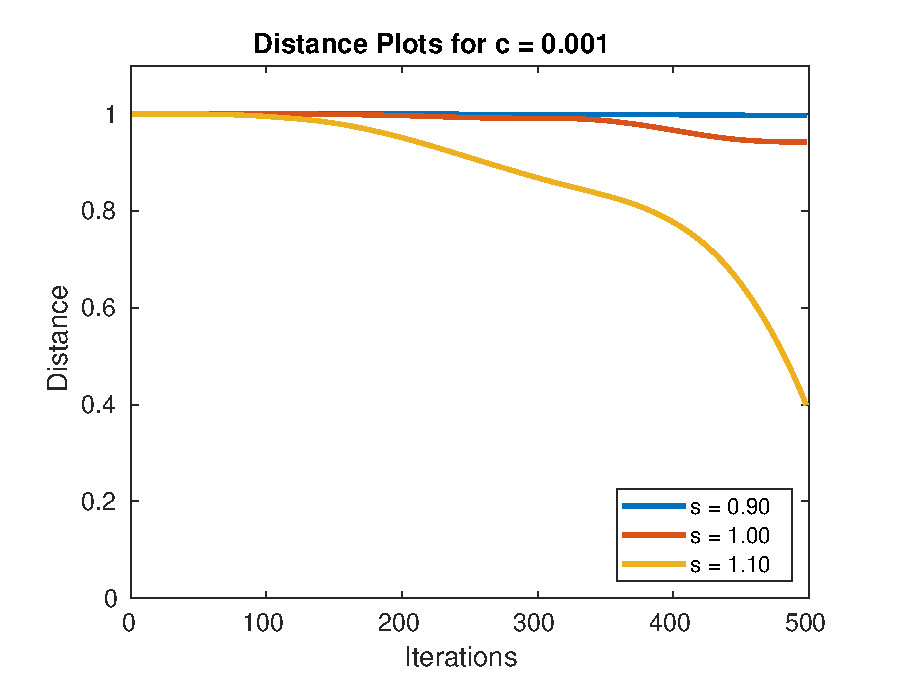
\epsfig{file=new_figures_c_0_001.eps,width=2.63in,height=1.68in}} 
{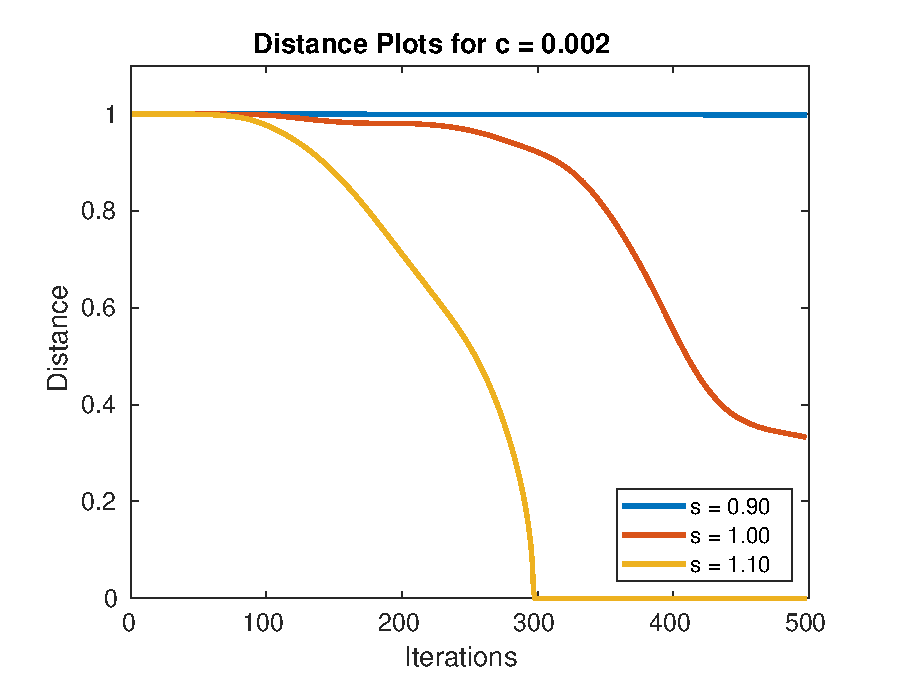
\epsfig{file=new_figures_c_0_002.eps,width=2.63in,height=1.68in}} 
\vspace{5mm}
{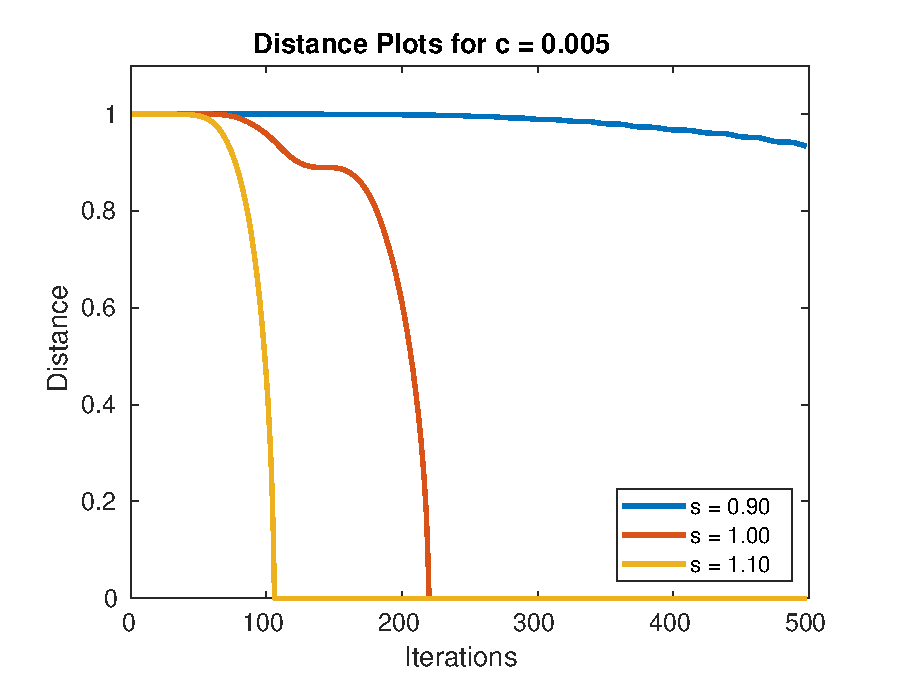
\epsfig{file=new_figures_c_0_005.eps,width=2.63in,height=1.68in}} 
{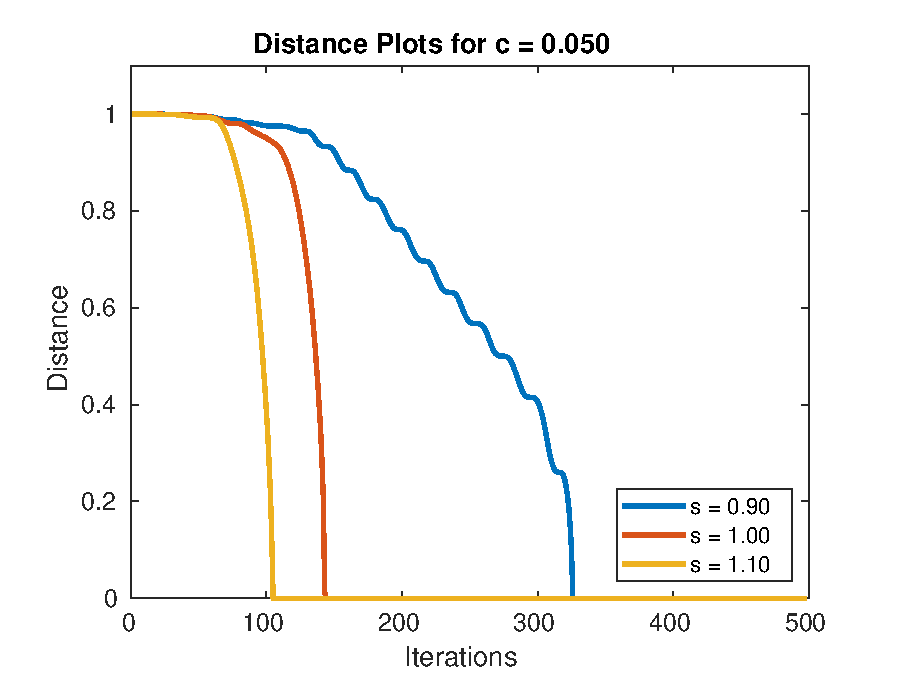
\epsfig{file=new_figures_c_0_050.eps,width=2.63in,height=1.68in}} 
\caption{}
\end{figure}

%\begin{figure}[h]
%\centering
%{\epsfig{file=compare_c_0_001.eps,width=2.63in,height=1.68in}} 
%{\epsfig{file=compare_c_0_002b.eps,width=2.63in,height=1.68in}} 
%\vspace{5mm}
%{\epsfig{file=compare_c_0_005.eps,width=2.63in,height=1.68in}} 
%{\epsfig{file=compare_c_0_050c.eps,width=2.63in,height=1.68in}} 
%\caption{}
%\end{figure}

%\begin{figure}
%\centering
%\includegraphics[scale=0.35]{Fig1_version2}
%\caption{}
%\end{figure}

%\begin{figure}
%\centering
%\includegraphics[scale=0.35]{fig2a_version1}
%\caption{}
%\end{figure}

%\begin{figure}
%\centering
%\includegraphics[scale=0.35]{fig2b_version1}
%\caption{}
%\end{figure}

%\begin{figure}
%\centering
%\includegraphics[scale=0.35]{fig2c_version1}
%\caption{}
%\end{figure}

%\subsubsection{Sub-diffusion}

%\begin{figure}[H]
%\centering
%{\epsfig{file=sub_compare_c_0_001.eps,width=2.63in,height=1.68in}} 
%{\epsfig{file=sub_compare_c_0_002.eps,width=2.63in,height=1.68in}} 
%\vspace{5mm}
%{\epsfig{file=sub_compare_c_0_005.eps,width=2.63in,height=1.68in}} 
%{\epsfig{file=sub_compare_c_0_050a.eps,width=2.63in,height=1.68in}} 
%\caption{}
%\end{figure}

%\subsubsection{Super-diffusion} 

%\begin{figure}[H]
%\centering
%{\epsfig{file=sup_compare_c_0_001.eps,width=2.63in,height=1.68in}} 
%{\epsfig{file=sup_compare_c_0_002.eps,width=2.63in,height=1.68in}} 
%\vspace{5mm}
%{\epsfig{file=sup_compare_c_0_005.eps,width=2.63in,height=1.68in}} 
%{\epsfig{file=sup_compare_c_0_050.eps,width=2.63in,height=1.68in}} 
%\caption{}
%\end{figure}

%\josh{I need the original figure files to import in to \LaTeX...}

%\subsubsection{Correlation Induced Transport at Nonzero Disorder}

%\no\josh{We haven't discussed any ideas in this direction, so we should maybe remove this section...}

%\subsubsection{``Range" of Anomalous Interaction}

%\josh{Do we want to mention here how various truncations of the formal sum may be viewed as true approximations of some ``nearby" nonlocal operator? Or do we simply want to formulate this as an exploration of the effects of truncation, without some reference to a possibly deeper mathematical interpretation?}

\subsection{Interpretations and Limitations}

\no\josh{This will include a brief discussion on the ``influence" issues that we have discussed in great length...}

\subsection{Orthogonality Check}

\no\josh{I will briefly include a description of the Lanczos algorithm here. There will also be a table depicting the various outputs of the algorithm (which are all outputs very close to zero--on the scale of $10^{13}$ to $10^{14}$...}

\section{Conclusions and Future Work}

\noindent\josh{I will update this later...}

\subsection{Connection with Lie Algebraic Formulations and Quantum Mechanics}

%\josh{This will require some thinking on my part. The hope is not to just frivolously consider Lie algebras for this problem in hopes of making a blind connection. We will need to consider exactly what algebraic structure is hoping to be uncovered. For instance, if we know that physically systems exhibiting localization have some algebraic properties or even symmetries, then this becomes an easier question to answer...We can surely find SOME Lie algebraic setting for the problem, but the key is to find a USEFUL/MEANINGFUL algebraic setting.}

%\josh{I think the primary question here is what invariant properties are typically present in localization problems?}

\no\josh{We haven't discussed any ideas in this direction, so we should maybe remove this section...}

\subsection{Application to Strongly Coupled Coulomb Systems}

\no\josh{This needs double checking...}

Strongly correlated systems (SCSs) are systems that cannot be effectively described by the physics of free-particle ensembles. Instead, these systems exhibit anomalous (often technologically useful) collective behavior, which results from strong interactions between the involved entities \cite{gogolin2004bosonization,avella2012strongly}. Strong correlations characterize important observed phenomena in the fields of particle physics (hadron-meson interaction and quark-gluon plasma formation), materials science (electrical resistance of metallic magnets and high-temperature superconductivity), and biology (muscle cell excitation and protein folding) \cite{anisimov2010electronic,fulde2012electron,
quintanilla2009strong,zhang2008reentrant}. It has been recognized that the development of a comprehensive theoretical model for strong correlations which scales appropriately across various size and time scales is one of the most difficult and yet fundamental problems in modern physics \cite{gogolin2004bosonization,
quintanilla2009strong,kotliar2004strongly}.
Of particular interest to both the science community and industry is the dynamical behavior of unconventional superconductors such as heavy-fermion compounds \cite{pfleiderer2009superconducting}, organic superconductors \cite{ishiguro2012organic}, and iron cuprates \cite{stewart2011superconductivity}. Despite the remarkable advancements in the experimental characterization of such materials, the theoretical explanation of unconventional superconductivity has proven challenging. One reason is that the experimentally studied strongly correlated materials are generally very complex, multi-layered crystals (for instance, BSCCO), which makes numerical modeling difficult and the growth of high quality crystalline samples expensive. Such difficulties have motivated the development of simplified SCSs, which exhibit analogous interactions in a controlled environment. One possible approach is the use of strongly correlated ultracold atoms (fermions) trapped in optical lattices, which have been shown to exhibit anomalous diffusion effects \cite{barkai2014area,kessler2012theory,mazurenko2017cold}. An important disadvantage of cold-atom systems is the effective lack of lattice disorder, which plays an important role in the transport properties of most crystals \cite{polini2013artificial}. Another solution is offered by the fast-growing field of complex (dusty) plasmas, where the interparticle interaction is often characterized by a Yukawa (or shielded-Coulomb) potential. Superdiffusion has been investigated numerically in two-dimensional \cite{liu2007superdiffusion,ott2009anomalous,liu2006test} and quasi-two-dimensional \cite{ott2008superdiffusion} Yukawa liquids. Experimentally, deviations from classical diffusion have been observed in driven-dissipative two-dimensional dusty plasma \cite{liu2008superdiffusion}.

Besides the need for optimization of simplified crystal analogues, the theory of superconductivity (and, in general, strong correlations) lacks a sound mathematical formulation that scales appropriately for the variety of SCSs found in nature. The implementation of the fractional Laplacian model for anomalous diffusion due to strong correlations is an important step in the development of such theory. The focus of our future work will be optimization and generalizations of the numerical techniques presented herein. The numerical predictions will be experimentally verified using a SCSs analogue system and then compared to experimental studies of superconductor materials.

\begin{itemize}
\item[\josh{5.}] \josh{It would be nice if we could break this first paragraph in this section up since it is a little long, but this is in no way necessary.}

\item[\josh{6.}] \josh{I will need the physics crowd to proofread the above, as this is a bit outside of my expertise...}
\end{itemize}

\section*{Acknowledgments}

\noindent This work was supported by the NSF-DMS, grant number 1802682 (CDL), NASA, grant number 1571701 (LSM and TWH), NSF/DOE Grant numbers 1414523, 1707215 (LSM and TWH), and NSF Grant Number 174023 (LSM and TWH). 
%\josh{The physics grants are good...Need to ask Conni...}

\section*{References}

%\begin{itemize}
%\item[\josh{6.}] \josh{We have quite a few references...I would say we need to make sure that each of them is actually necessary...}

%\item[\josh{7.}] \josh{I have proofread the references, but it is always helpful to have someone else go over them to see if there are any other typos or formatting errors...}
%\end{itemize}

\bibliographystyle{plain}
\bibliography{Anderson_Bib}

%% else use the following coding to input the bibitems directly in the
%% TeX file.

%\begin{thebibliography}{00}

%% \bibitem[Author(year)]{label}
%% Text of bibliographic item

%\bibitem[ ()]{}

%\end{thebibliography}

%5\appendix
%\section{Proof of Theorem 2.i.}

%\josh{I will further improve the description here...}

%We now provide the proof to Theorem 2.{\em i.} The proofs of the remaining parts are technical, yet similar to those in \cite{ciaurri2015fractional,ciaurri2016nonlocal}, so we will postpone the details for our future work.



\end{document}

\endinput
%%
%% End of file `elsarticle-template-harv.tex'.
